\documentclass{article}

% --- load packages ---

\usepackage[margin=1in]{geometry} % change the margins
\usepackage{amsmath} % useful math environments and commands like align
\usepackage[colorlinks,bookmarks,bookmarksnumbered,allcolors=blue]{hyperref} % hyperlinks between references
\usepackage{graphicx}  % include images
\usepackage[caption=false]{subfig} % subfigures.  false option prevents conflicts in caption styling with other packages
\usepackage{booktabs} % better tables
\usepackage[capitalise]{cleveref} % better referencing. uses cref.
\usepackage[section]{placeins} % sometimes useful to prevent figures from floating out of a section
\usepackage{cite} % handles multiple citations in one command better
\usepackage{doi} % allow correct hypderlinking of DOIs

\newcommand{\code}[1]{\texttt{#1}}

\begin{document}

\title{ME 575 --- Homework 3}
\author{Seth Nielsen}
% put in \date{} if you don't want a date to appear, or enter a specific date, otherwise default is today's date.
\date{}
\maketitle

\section*{Introduction}

For this assignment, I worked on optimizing the same 10-bar truss problem from the first homework, but with the gradients for the objective and the contraints provided by my own algorithms. I did the assignment entirely in Python 3. The following four approaches were used for computing the gradients:

\begin{enumerate}
	\item Forward-difference
	\item Complex-step
	\item Forward-mode autodifferentiation (provided by Google's \texttt{JAX} library)
	\item Analytic adjoint
\end{enumerate}

\section{Truss Derivatives}

Let $A$ be the array containing the cross-sectional areas of the ten bars that make up the truss. Let $m$ be the total mass of the truss. Let $\sigma$ be the array containing the stress on each of the ten bars. The derivatives calculated by each of the four methods were:
\begin{itemize}
	\item $ \displaystyle \frac{dm}{dA} $ --- mass with respect to each cross-sectional area (array of size 10)
	\item $ \displaystyle \frac{d\sigma}{dA} $ --- all stresses with respect to each cross-sectional area (2D-array of size 10$\times$10)
\end{itemize}

The 

\begin{figure}[htbp]
	\begin{center}
		% 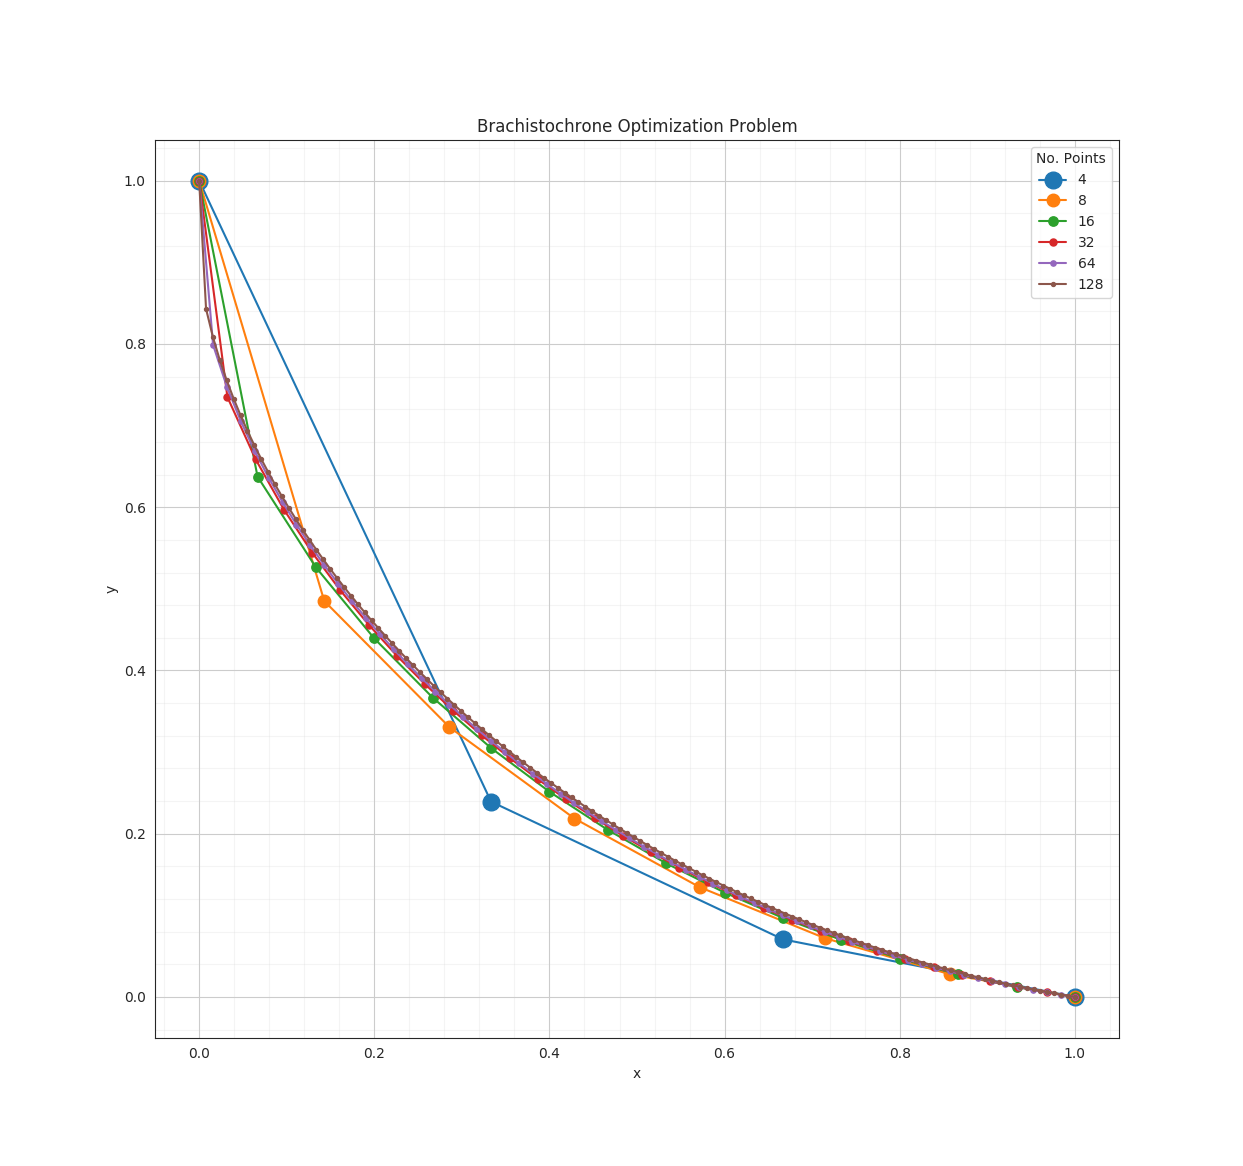
\includegraphics[width=0.75\textwidth]{figures/curve.png}
		\caption{\label{fig:brachcurve}}
	\end{center}
\end{figure}

\begin{figure}[htbp]
	\centering
	% 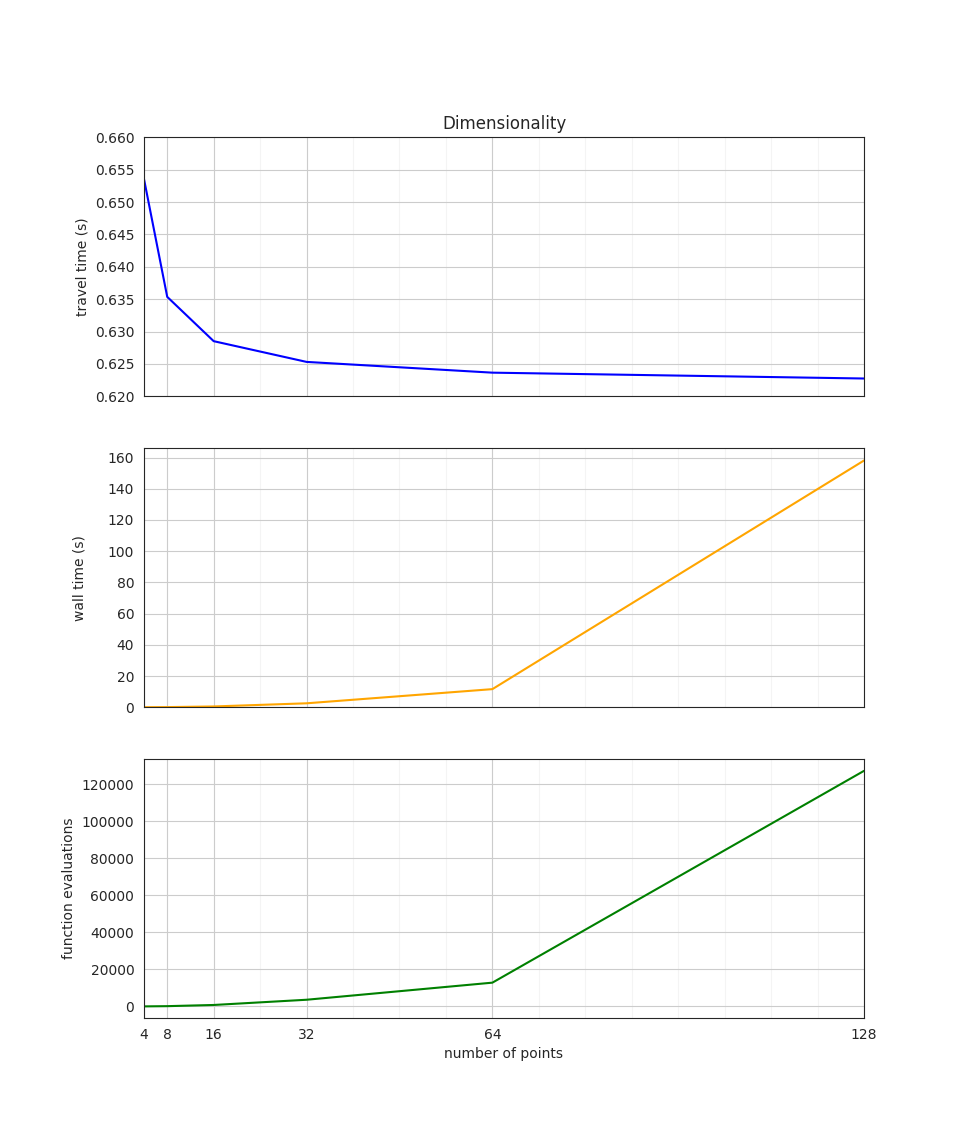
\includegraphics[width=0.75\textwidth]{figures/dimensions.png}
	\caption{\label{fig:dimensions}}
\end{figure}


\section{Truss}
It is interesting to note that bar 9, the bar made of the strongest material, was allowed to have the highest stress of any of the bars.

\begin{table}[htb]
	\begin{center}
		\caption{Comparison of number of function calls required for convergence.\label{tab:mytable}}
		\begin{tabular}{c c c c}
			\toprule
			\textbf{Algorithm} & Matyas & Rosenbrock & Brachis. \\
			\midrule
			\textbf{Custom} & 7.9 & 25e3 & 0 \\
			\textbf{pyOptSparse: SNOPT} & 0.14 & 11309 \\
			\bottomrule
		\end{tabular}
	\end{center}
\end{table}

\begin{figure}[htbp]
	\centering
	% 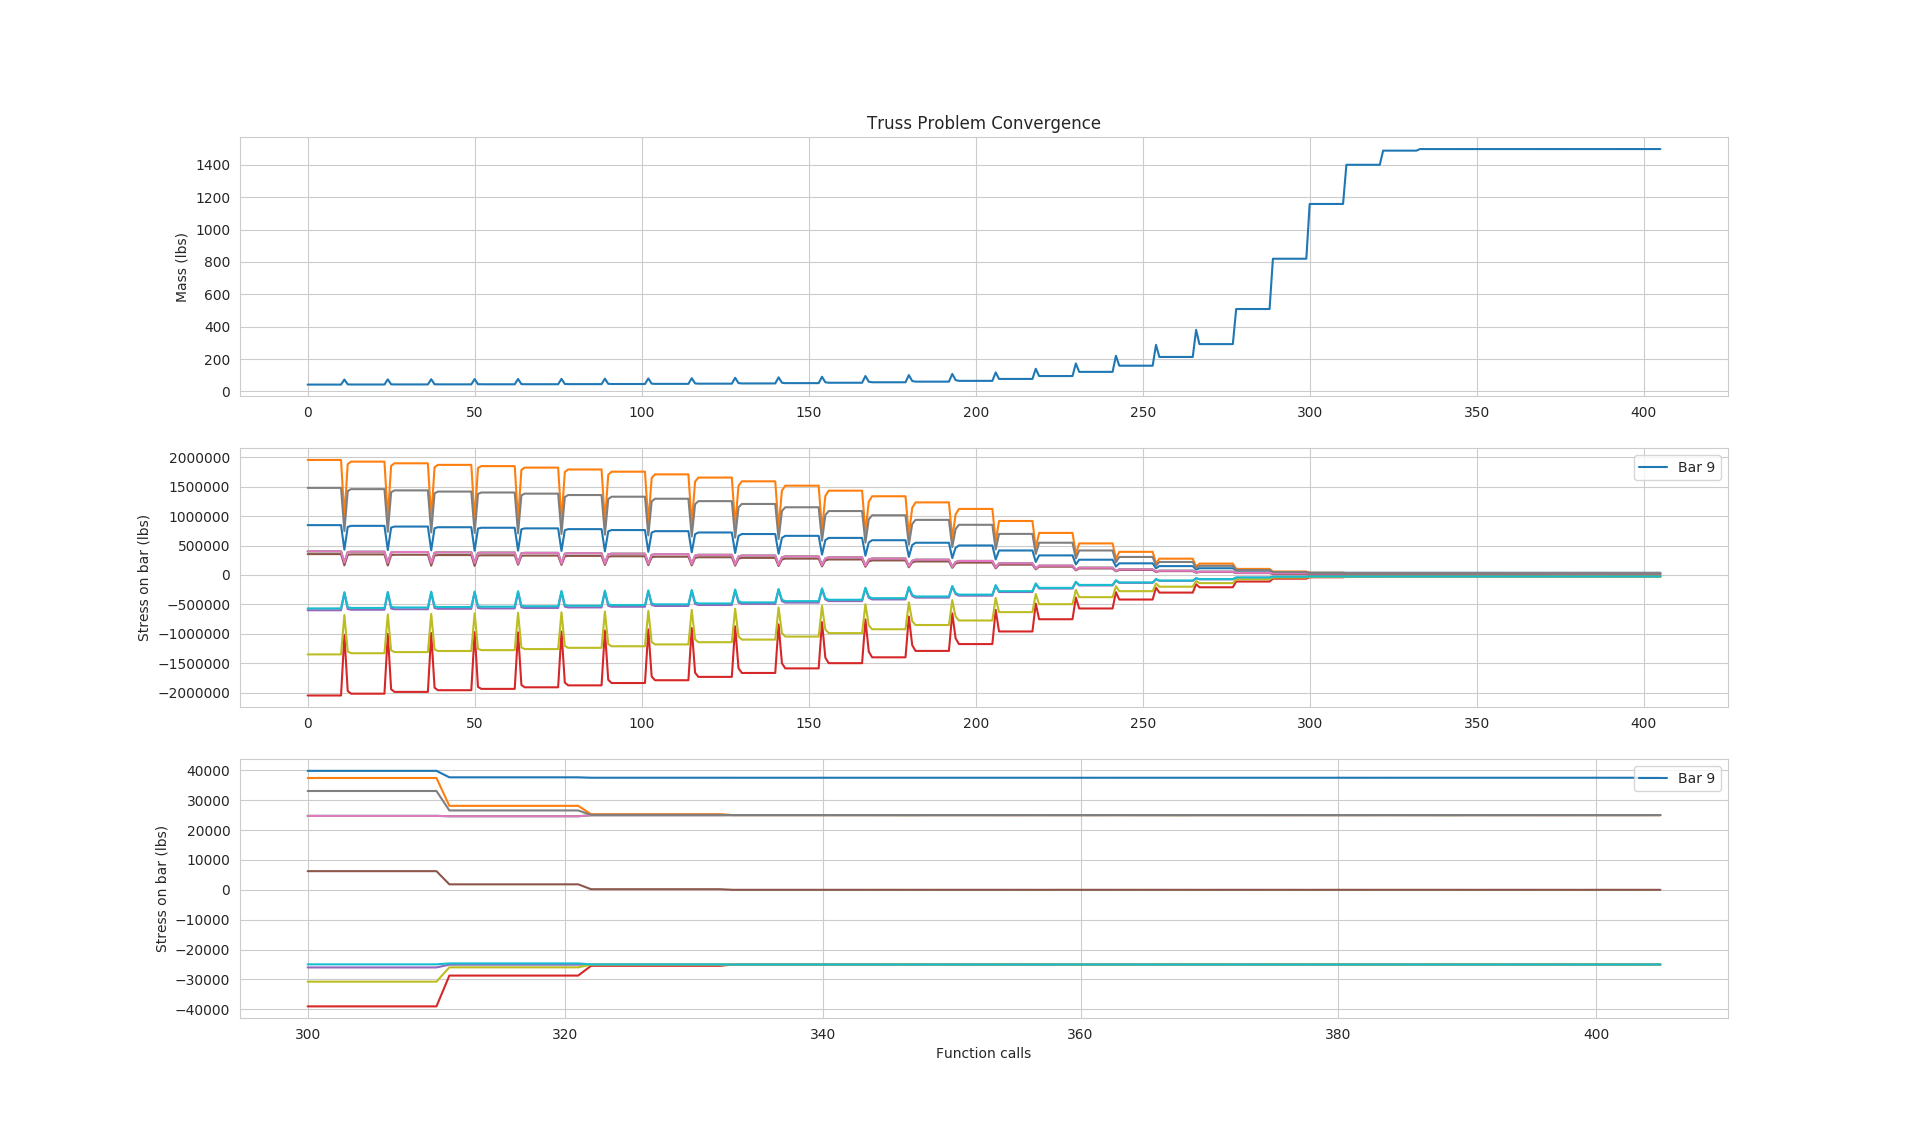
\includegraphics[width=0.75\textwidth]{figures/truss_plot.png}
	\caption{Convergence of objective value over function evaluations. The bottom plot is the same as the middle, but zoomed in for clarity.\label{fig:results}}
\end{figure}

% This is for the bibliography.  Note that it is using sample.bib
% you would need to provide your own bibtex file.

\end{document}